%% Beispiel-Präsentation
\documentclass{sdqbeamer}
 
%% Titelbild
\titleimage{banner_2020_kit}

%% Gruppenlogo
\grouplogo{hci}

%% Gruppenname und Breite (Standard: 50 mm)
\groupname{Mensch-Maschine-Interaktion und Barrierefreiheit}
%\groupnamewidth{50mm}

% Beginn der Präsentation

\title[Solidarische Raumnutzung Entwurfsheft]{Kolloquium Entwurfsheft zur Solidarischen Raumnutzung}
\author[Soli-Gruppe]{Alexander Klee, Jannik Hönlinger, Johannes Frohnmeyer, Ben Steinle und Antonia Ammon }
\subtitle{PSE-Projekt WS24/25}
\date[03.\,01.\,2025]{03. Januar 2025}

% Literatur
 
\usepackage[citestyle=authoryear,bibstyle=numeric,hyperref,backend=biber]{biblatex}
\addbibresource{presentation.bib}
\bibhang1em

\begin{document}
 
%Titelseite
\KITtitleframe

%Gliederung
\begin{frame}{Gliederung}
\tableofcontents
\end{frame}

\section{Aufbau}

\subsection{Architektur}
\begin{frame}{Architektur}
% add picture figures/Architektur.png
\begin{figure}
    \centering
    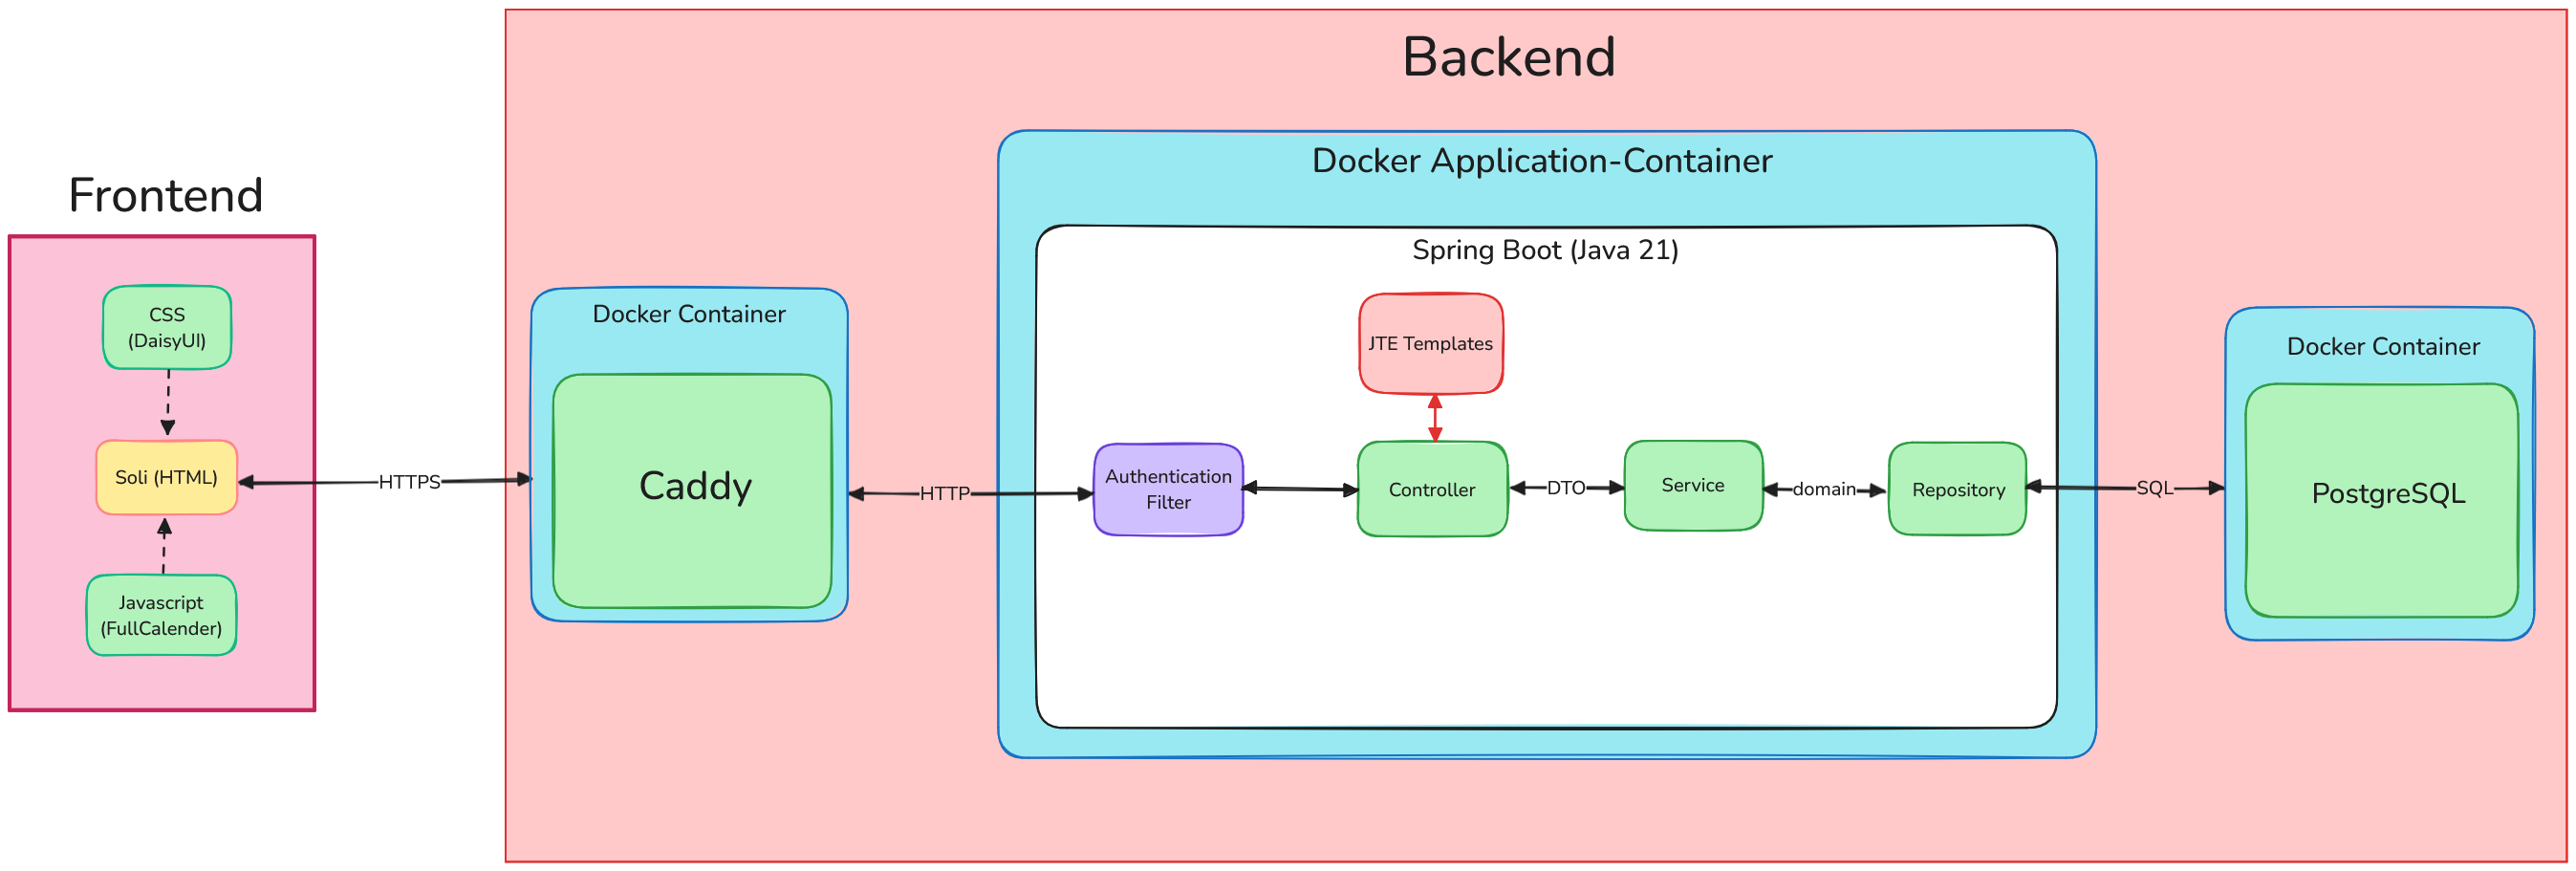
\includegraphics[width=\textwidth]{pictures/figures/architecture}
    \label{fig:architektur}
\end{figure}
\end{frame}

\end{document}